\documentclass[Report.tex]{subfiles}
\begin{document}

\chapter{Implementation}
In Chapter 2, the general flow of the processes between the different Python modules was described. Figure \ref{fig:sequence} shows in finer detail the order of the function calls from the \texttt{controller} module. The lifelines in sequence diagrams usually represent the creation and destruction of objects, however Object-Orientated programming was not used in this project. Therefore it can be assumed that the modules are only in use whilst the function calls are being carried out. In this chapter, the details of each process of the application are discussed to explain the reasoning behind the technologies chosen, and to analyse how well each component functions.

\begin{figure}[h!]
\includegraphics[width=0.9\textwidth]{../lib/images/sequence.png}
\caption{Schematic of the key processes of the system, as explained in the text.}
\label{fig:sequence}
\end{figure}

\section{The Python Programming Language}
\subsection{Language Features}
Python is a dynamically typed, multi-paradigm language with an extensive package system outside of the standard library that anyone can add to, due to the open source nature of the Python source code\cite{pythonabout}. It was chosen due to its ease of use and applicability for a wide variety of tasks, including HTTP request handling, unit testing and JSON encoding/decoding. Throughout this project, I have found these and modules such as \texttt{subprocess} for spawning a MetaMap process, and external libraries such as BioPython for submitting Entrez requests, extremely useful for the tasks at hand. The usage of BioPython was not strictly necessary, as the E-Utils are accessible via simple HTTP requests. However, BioPython automates many of the finer tunings, ensuring that the query rate is not greater than 3 per second (source code available at \url{https://github.com/biopython/biopython/blob/master/Bio/Entrez/} and documentation at \url{http://biopython.org/DIST/docs/api/}). This is the greatest strength of Python - if a tool has not already been made by the active community of developers, it is possible, and encouraged, for one to build a new library themselves.

\subsection{Project Structure}
\noindent That Python programs do not explicitly require a structure is one of its strengths - but also a potential downfall for inexperienced developers. Modules can be organised into packages with the inclusion of a \texttt{\_\_init\_\_.py} file, but even this is optional. It was difficult to know how to structure the application, particularly with the usage of the Flask microframework. However with the popularity of MVC-like frameworks such as Django and Ruby on Rails it was not difficult to find comparable projects to base the directory structure of the application on. It is also largely down to the personal preference of the developer, and does not impact the performance of the application at all. Within modules, there is a choice to be made between keeping the module as a collection as functions, or turning it into a Class to utilise object-orientated programming principles and patterns. In a language such as Java or Ruby, I most likely would have created a Citation class with attributes for important fields such as PMIDs, and written getters for each. In Python, this style of programming is possible but perhaps overwrought considering the ease with which Python handles JSON objects and decodes them into dicts. Each PubMed entry has a large number of fields, so would have required complicated objects (with a number of fields set to null, as few elements are mandatory) to fully represent all citation types. Citation objects were left as JSON objects/Python dicts to decrease the overhead of object creation, and also to simplify the passing of messages between modules, at the cost of a better defined structure. 

\subsection{The Flask Microframework}
 Flask is extremely lightweight, requiring minimal input to produce a basic server that can route requests from the client. This was perfect for the simplicity of the application, that currently does not require user or admin accounts and the associated security risks and storage implications. Though a cache was eventually implemented, this is external to the core of the framework as all input comes from the backend. 

\section{Searching For Concepts Using MetaMap}
\subsection{The Utility of MetaMap}
Due to the problems of Word-Sense Disambiguation in natural language processing, it was assumed that directly searching the UMLS for concepts would not have a high success rate. For example, a title such as \emph{"Loss of SMAD4 Promotes Colorectal Cancer Progression by Accumulation of Myeloid-Derived Suppressor Cells through CCL15-CCR1 Chemokine Axis"} contains composite phrases e.g. "cancer progression" that confer additional information together as opposed to when processed separately. This semantic analysis is would be challenging to implement manually and would most likely result in inaccuracies.

\subsection{MetaMap vs. The MTI}
\noindent MetaMap can be invoked either locally or via the Semantic Knowledge Representation Web API within the MTI. Both options were tested to compare performance. The MTI results are more refined (see Table \ref{tab:mm-results}), and consequently produce concept visualisations that are easier to understand (Figure \ref{fig:mm-screen}). Compared to the visualisation in Figure \ref{fig:screen1} produced using the MTI, there are more nodes, and many co-occur in the same hierarchies, suggesting some data redundancy. In Table \ref{tab:mm-results} it can be seen that MetaMap alone produced a higher number of results, some of which were inaccurate. For example, the phrase \emph{"Chemokine Axis"} appears to have been incorrectly interpreted by MetaMap to consist of two separate terms, hence the return of the concept \emph{"Axis vertebra"} (MetaMap, concept 3). For these reasons, the MTI was determined to be a better fit for this project. However the performance difference is not trivial. On a standard broadband connection, the full MTI process takes around 5-10 minutes. This is in contrast to running MetaMap locally, the output of which is delivered after less than a minute. It was decided to keep both options in the source code as \texttt{metamap.run} and \texttt{metamap.run\_local}, respectively, but to only include the abstract text for the remote service, as inclusion results in an excessive number of concepts with the local service. Both methods use the \texttt{subprocess} Python module and return results in almost identical formats, so switching between the two is reflected in the concepts only.\newline

\begin{table}[!h]
\begin{center}
    \begin{tabular}{ | c | l | l | }\hline
    \textbf{\#} & \textbf{MTI concepts} & \textbf{MetaMap concepts}\\ \hline
1 & CCL15 protein, human & Axis\\ \hline
2 & \*Macrophage Inflammatory Proteins & Axis vertebra\\ \hline
3 & \*Chemokines, CC & chemokine\\ \hline
4 & \*Chemokines & Disease Progression\\ \hline
5 & \*Colorectal Cancer & CCL15 protein, human\\ \hline
6 & \*Disease Progression & Genus Axis\\ \hline
7 & \*Neoplastic Processes & Promotion (action)\\ \hline
8 & \*Neoplasms & Loss\\ \hline
9 & Receptors, CCR1 & Progression\\ \hline
10 & \*Antigen Presentation & CCL15 gene\\ \hline
11 & immunology & CCR1 gene\\ \hline
12 & - & Chemokine (C-C Motif) Receptor 1\\ \hline
13 & - & SMAD4 gene\\ \hline
14 & - & Cancer Genus\\ \hline
15 & - & Cells\\ \hline
16 & - & Cells [Chemical/Ingredient]\\ \hline
17 & - & Colorectal\\ \hline
18 & - & Derivation\\ \hline
19 & - & Derived value\\ \hline
20 & - & Malignant Neoplasms\\ \hline
21 & - & Myeloid\\ \hline
22 & - & Primary malignant neoplasm\\ \hline
23 & - & Suppressor\\ \hline
24 & - & Suppressor Device Component\\ \hline
    \end{tabular}\\
    \caption{Output from MetaMap and MTI for the title \emph{"Loss of SMAD4 Promotes Colorectal Cancer Progression by Accumulation of Myeloid-Derived Suppressor Cells through CCL15-CCR1 Chemokine Axis"}.}
\label{tab:mm-results}
\end{center}
\end{table}
\begin{figure}[h!]
\begin{center}
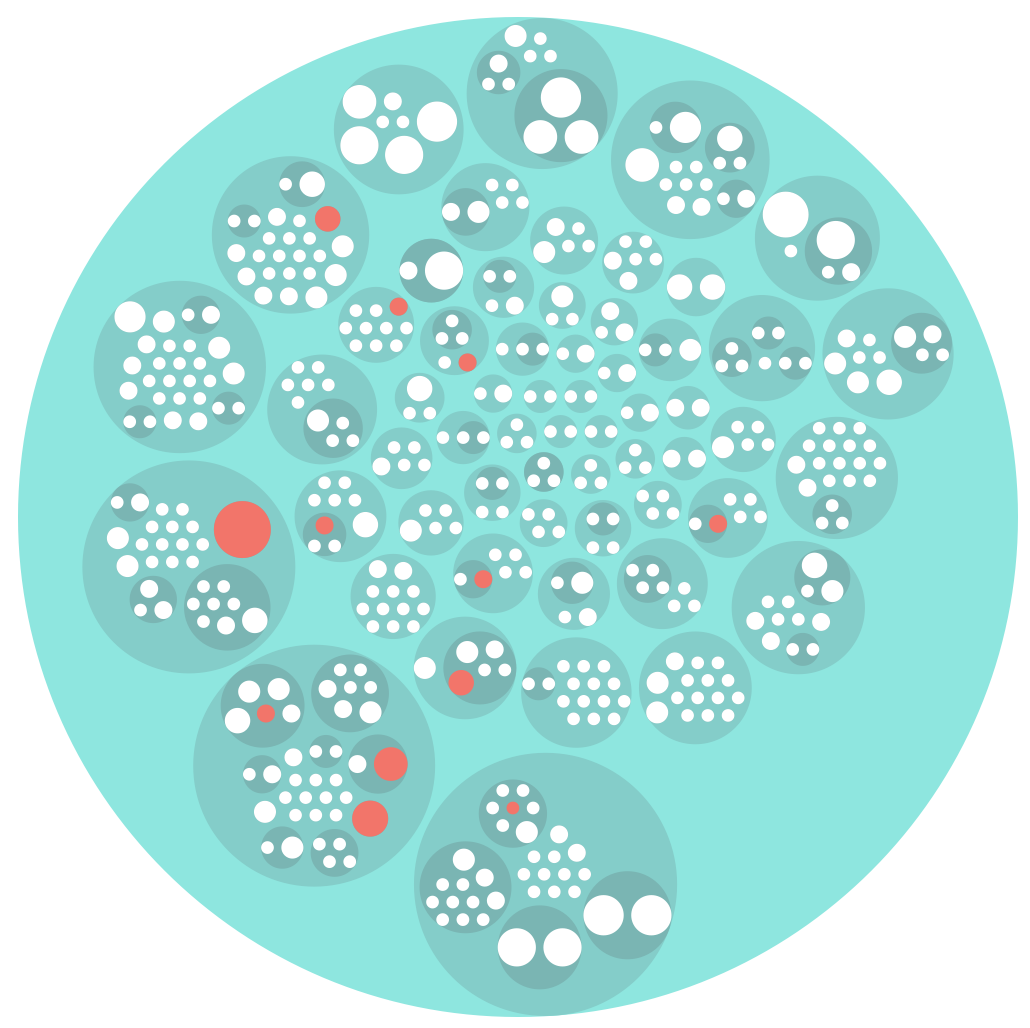
\includegraphics[width=0.4\textwidth]{../lib/images/mm-screen.png}
\caption{The concept visualisation from the search term 'computer' using local MetaMap.}
\label{fig:mm-screen}
\end{center}
\end{figure}\newpage

\section{Organising Concepts Into Hierarchies Using The MetaThesaurus}
\subsection{MetaThesaurus Setup}
The MetaThesaurus is free to download from the NIH (available from \url{http://www.nlm.nih.gov/research/umls/licensedcontent/umlsknowledgesources.html}) with a valid UMLS Terminology Services account. The NIH provides database subsets for Microsoft Access, Oracle or MySQL Relational Database Management Systems. MySQL was chosen to the proprietary nature of Access and Oracle. During installation, 70 vocabularies were chosen for inclusion based on the MetaThesaurus defaults and the language specified, which was restricted to English. These are listed in Appendix B, Table \ref{tab:vocabs}. 

\subsection{Querying MySQL}
An external library, PyMySQL, was used to execute SQL queries from the \texttt{umls} module. A summary of the database schema is shown in Figure \ref{fig:db}, showing only the attributes and tables necessary for the query. The query (Appendix A, page ???) receives a list of CUIs as input and returns the Semantic Type (from \texttt{MRSTY} as well as any direct parents. Direct parent concepts are defined as having a \texttt{MRREL.RELA} relationship of 'inverse\_isa'. This was chosen due to its explicit mapping of a parent/child hierarchy, and as a result of investigating similar options \texttt{MRREL.REL} = 'RB' (broader relationship) and \texttt{MRREL.REL} = 'PAR' (parent) that return results that were not true 'isa' relationships. Not all concepts have an 'inverse\_isa' relationship, and therefore outer joins were used to allow null values. Each concept has at least one Semantic Type.

\begin{figure}[h!]
\begin{center}
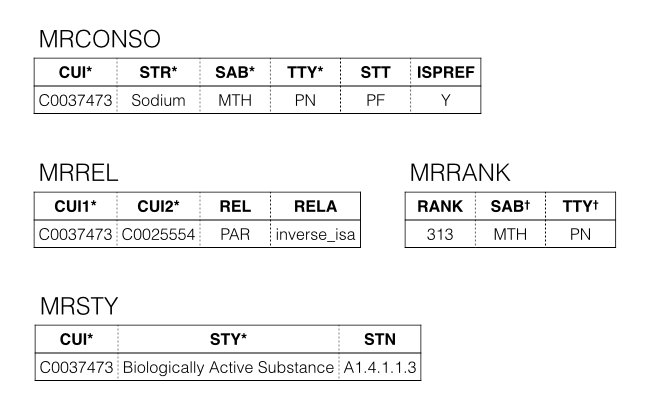
\includegraphics[width=0.7\textwidth]{../lib/images/db.png}
\caption{Attributes and tables used in the SQL query to retrieve concepts, their direct parents, and their semantic types.}
\label{fig:db}
\end{center}
\end{figure}

\noindent Each concept is represented in multiple vocabularies, each with their own string. To standardise the nomenclature used as much as possible, only the name from highest ranked source for each CUI is used. Rankings are defined in \texttt{MRRANK}, and the default rankings were used. The top ranking is 313, held by the MetaThesaurus preferred names (\texttt{SAB} = 'MTH', \texttt{TTY} = 'PN'). It was discovered that there are 2,295,761 CUIs in the database, of which only 172,139 have a MTH/PN source. For this reason, it was decided not to restrict just to the top ranking vocabulary as this would exclude a large proportion of the dataset. Resulting rows are also ordered by Semantic Type tree numbers (\texttt{MRSTR.STN}) before the \texttt{GROUP BY}, so that only the node furthest up the hierarchy is used as a Semantic Type.\newline

\noindent After the SQL query has produced rows corresponding to the semantic types and direct parents of each concepts, this data can be formatted into nested Python dicts, ready for encoding as JSON objects for the client-side JavaScript functions. Example output from the \texttt{umls} module can be seen in Appendix B, page ???, when one paper was retrieved with the search term 'computer'. The remote MTI service was used to attain the concept IDs. There are some redundancies in data, for example both the Semantic Type and parent concept of 'computers' is 'Manufactured Object', however I think it is best to retain this structure, which may be informative if another concept also has the Semantic Type of 'Manufactured Object', but not the direct parent. Additionally, both child concepts 'Nurse' and 'Nursing Staff, Hospital' were produced by the MTI, though this overlap is difficult to solve without access to the internal workings of the MTI.

\section{Geocoding}
\subsection{Optimisation}
The overhead of geocoding an address for the first time is high; the Text Search service in the Google Places API returns the top ten results that match the input parameters. In order to try and make the results more precise, the 'types' parameter is provided to specify that results should be either a university, a hospital, or an 'establishment' which is set as the default if a type is not present. In order to maximise the number of meaningful results achieved by the API, the input must be optimised to improve the chance that any location is returned (from this point onward referred to as the 'hit rate') and accuracy of the geocoding process. A number of formatting options were empirically tested, enabling an informed decision to be made for the geocoding function in the application.\newline

\noindent In order to have confidence in applying these findings to the larger population of papers available on PubMed, a dataset with papers on a range of topics, from various journals, and originating from numerous countries was required. Statistics on the publishing distribution between countries was found on Medline Trend\cite{medlinetrend}, though the data was limited to a date range of 2008-2012. Table \ref{tab:countries} lists the ten countries with the most papers, their percentage share and the corresponding number of papers used in the dataset. Though the intention was to have the number of addresses reflect these data, each paper in the dataset has multiple affiliation addresses, skewing the distribution. Thus, the primary feature of the dataset is that each of these countries is represented at least once. 33 unique papers and 178 addresses were included to assess the hit rate, and 10 papers and 18 addresses were included to assess the accuracy. Expected locations were found manually using the Google Maps website, and therefore were tested at a smaller scale. The distance between the 'true' location and the geographical coordinates as returned by the Places API could then be compared. A radius of 5 kilometres was chosen as the cut-off distance for a location to be called as accurate. It is important to note that the allocation of correct addresses was somewhat subjective. Automation would have been preferred, however it was not possible to retrieve papers with exclusively the affiliation address in the query. Even if this could have been achieved, universities with campuses distributed over a large area may have produced misleading conclusions.\newpage

\begin{table}
\begin{center}
    \begin{tabular}{ | l | c | c | }\hline
    \textbf{Country} & \textbf{Papers (\%)} & \textbf{Papers in} \\
     & &\textbf{dataset}\\ \hline
    USA & 28.1 & 14\\ \hline
    China & 8.5 & 4\\ \hline
    United Kingdom & 7.7 & 4\\ \hline
    Japan & 5.8 & 3\\ \hline
    Germany & 5.1 & 3\\ \hline
    Italy & 3.7 & 2\\ \hline
    Canada & 3.5 & 2\\ \hline
    France & 3.5 & 2\\ \hline
    Australia & 2.6 & 1\\ \hline
    India & 2.6 & 1\\ \hline
    \end{tabular}
    \caption{Percentage share of published papers between 2008 and 2012 for the 10 countries with the highest values.\label{tab:countries}}
\end{center}
\end{table}

\noindent A number of formatting combinations were tested, as detailed in Figure \ref{fig:geoscatter}. As expected, there was an inverse correlation between the hit rate and the accuracy of geocoding; sending more information (a higher number of address lines, particularly at the start of the address) reduces the chance of a match to a location, however the location is more likely to be correct.\newline

\begin{figure}[!ht]
\begin{center}
	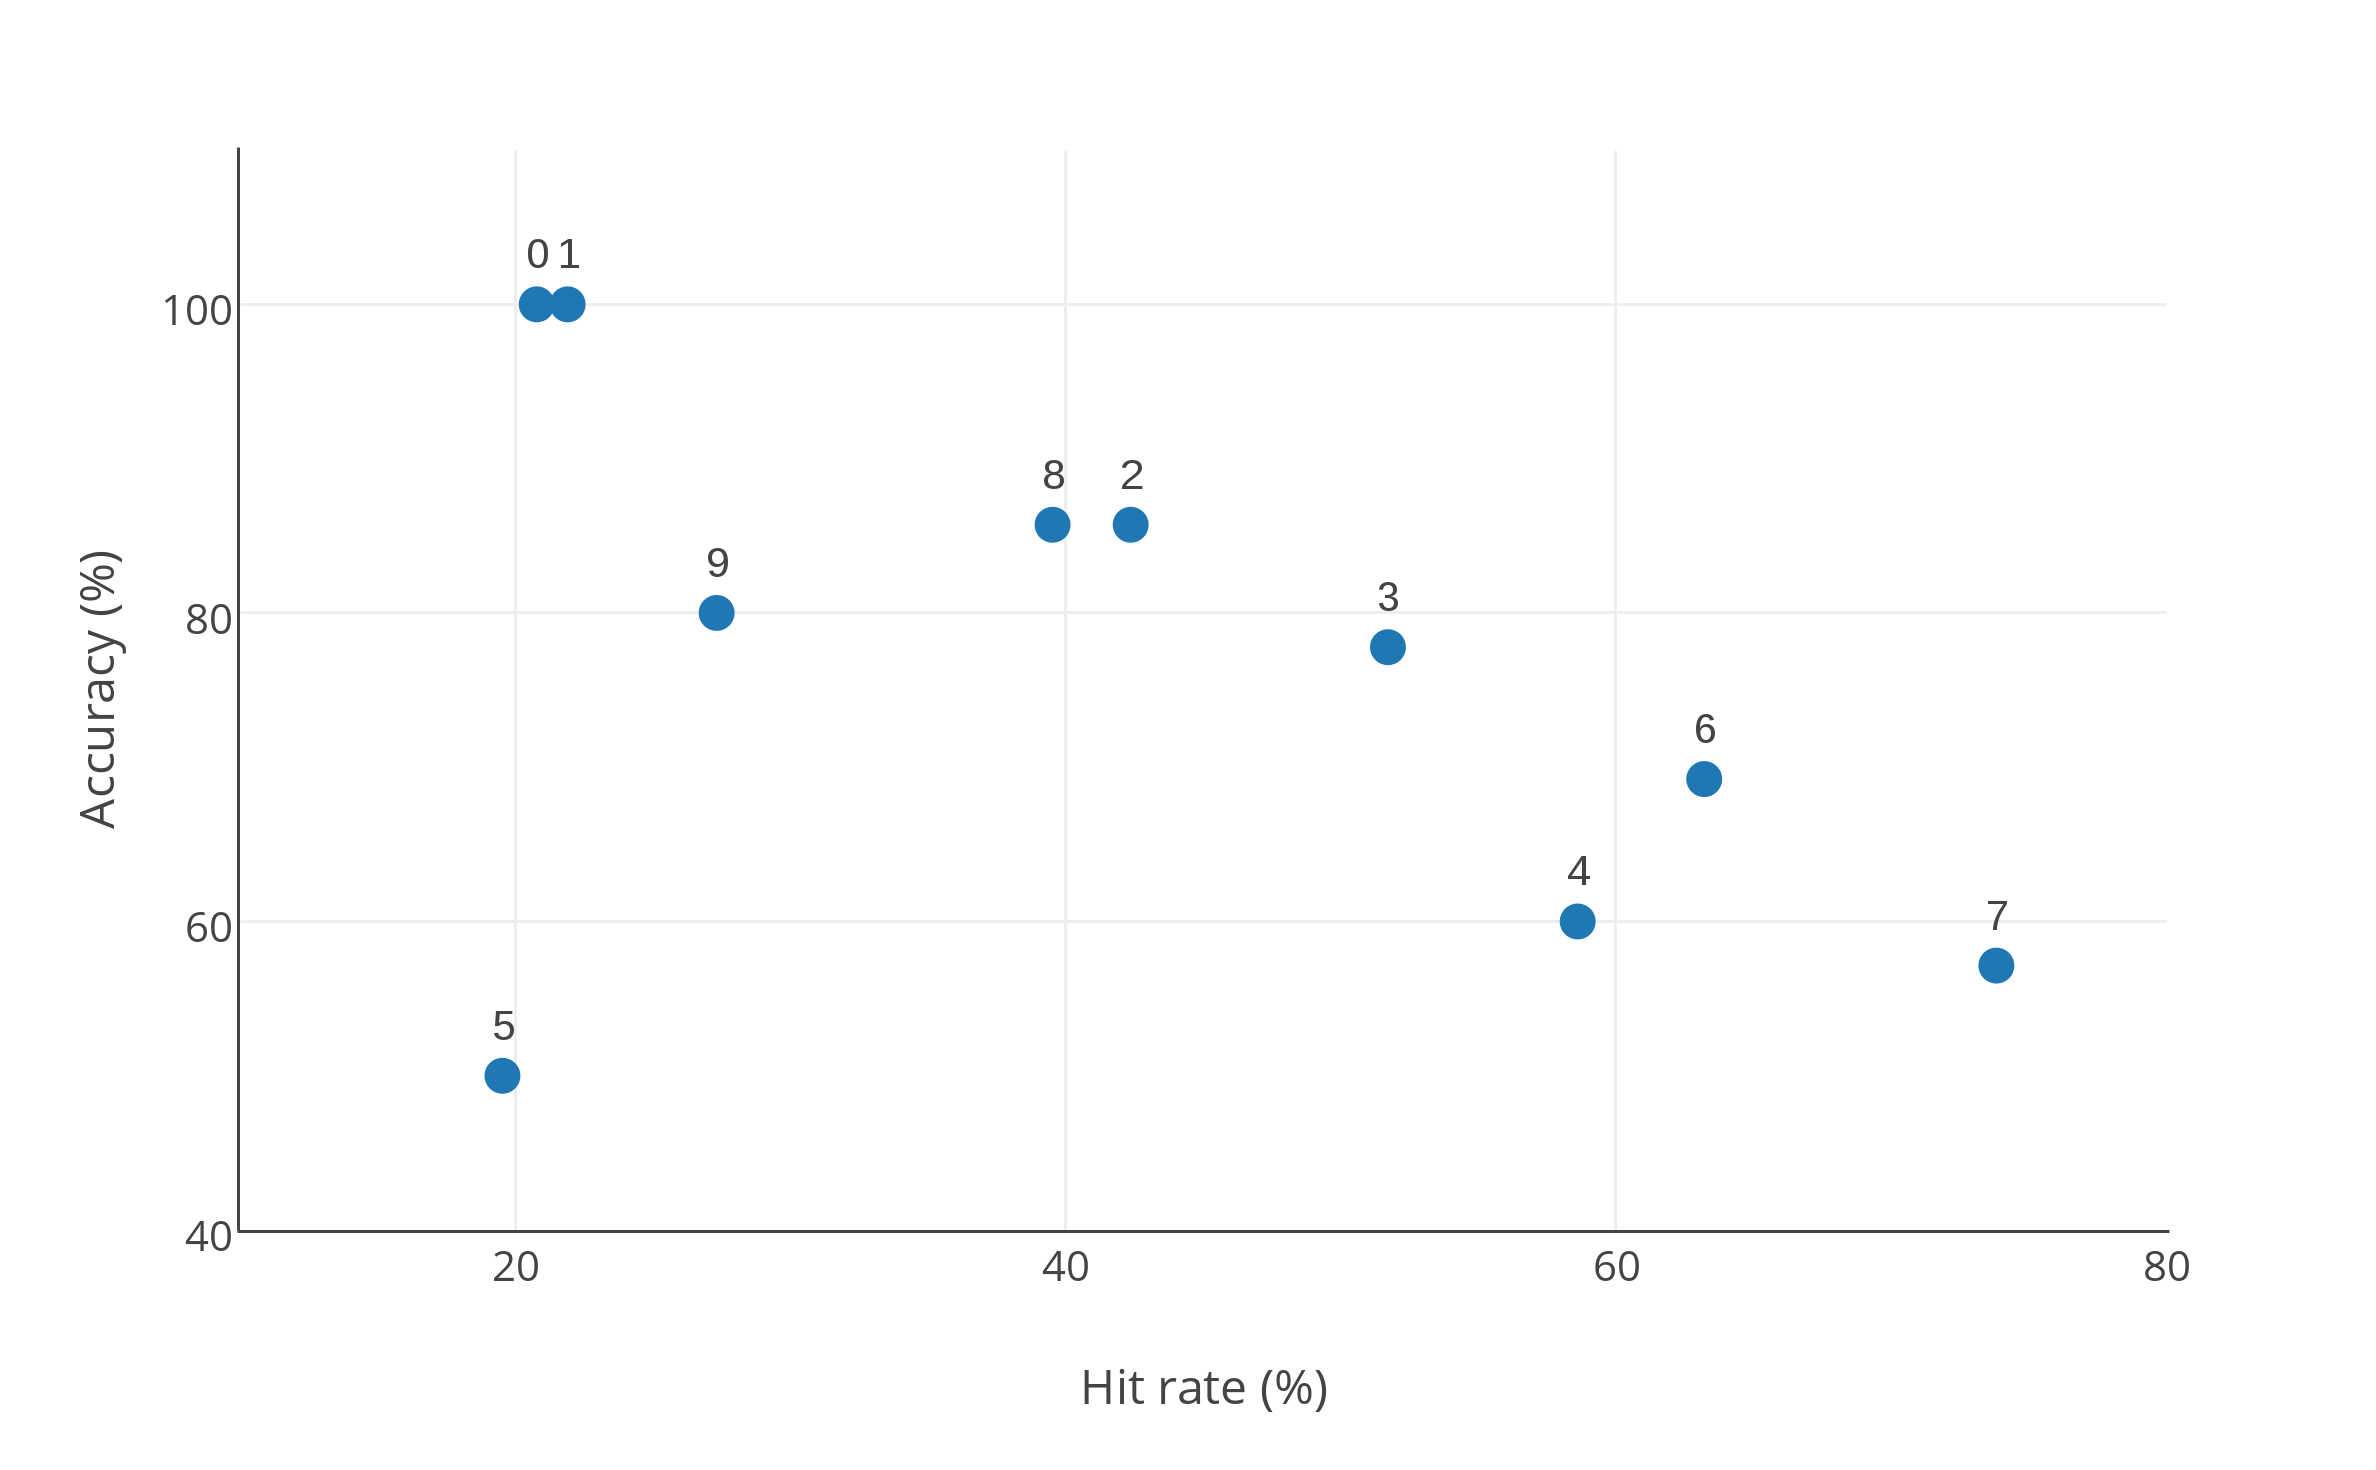
\includegraphics[width=0.8\textwidth]{../lib/images/geocode_performance_scatter}
	\caption{The hit rate (proportion of searches that returned any result, x-axis) and accuracy (proportion of searches that returned a result within 5 km of the expected loaction, y-axis) of 10 formatting options are plotted on this graph. The numbered points represent the following formats: 0 - none, 1 - email addresses removed, 2 - department removed, 3 - first line removed, 4 - department and first line removed, 5 - last 2 lines only, 6 - second and third lines only, 7 - second and last lines only, 8 - last 3 lines only, 9 - first 2 lines removed. Only options 0 and 1 include all addresses, as they are not limited by the number of lines in an address. \label{fig:geoscatter}}
\end{center}
\end{figure}

\noindent The first optimisations were carried out after observing trends during development. Email addresses of the lead author are sometimes included at the end of their affiliation address, which appeared to obfuscate the address for the Google Places API. Regular expressions were implemented from the \texttt{re} Python module in order to remove strings that matched the expected pattern for emails. As can be seen in Figure \ref{fig:geoscatter} (points 0 \& 1), removing email addresses did improve the hit rate of geocoding by 1\%. Of 15 addresses that contained email addresses, one (the Chinese Academy of Agricultural Sciences in Beijing) was matched to a location before removal of the email address. After formatting to remove the email address, 3 additional addresses were successfully matched to a location, however the Beijing address could not be matched. By checking the coordinates of the original returned address, it appears that the geocoding algorithm incorporated the email string to match the address to the Natural History Museum in London. In the accuracy dataset, 3 addresses included an email address but the hit rate was zero both before and after removal of the email address. From the incongruous result seen in the hit rate data, a tentative conclusion can be drawn that removing the email address improves the accuracy of results, though by a nominal amount. Spurious data was also seen elsewhere in the dataset, indicating that the input query can only be optimised to a certain degree.

\begin{figure}[!ht]
\begin{center}
	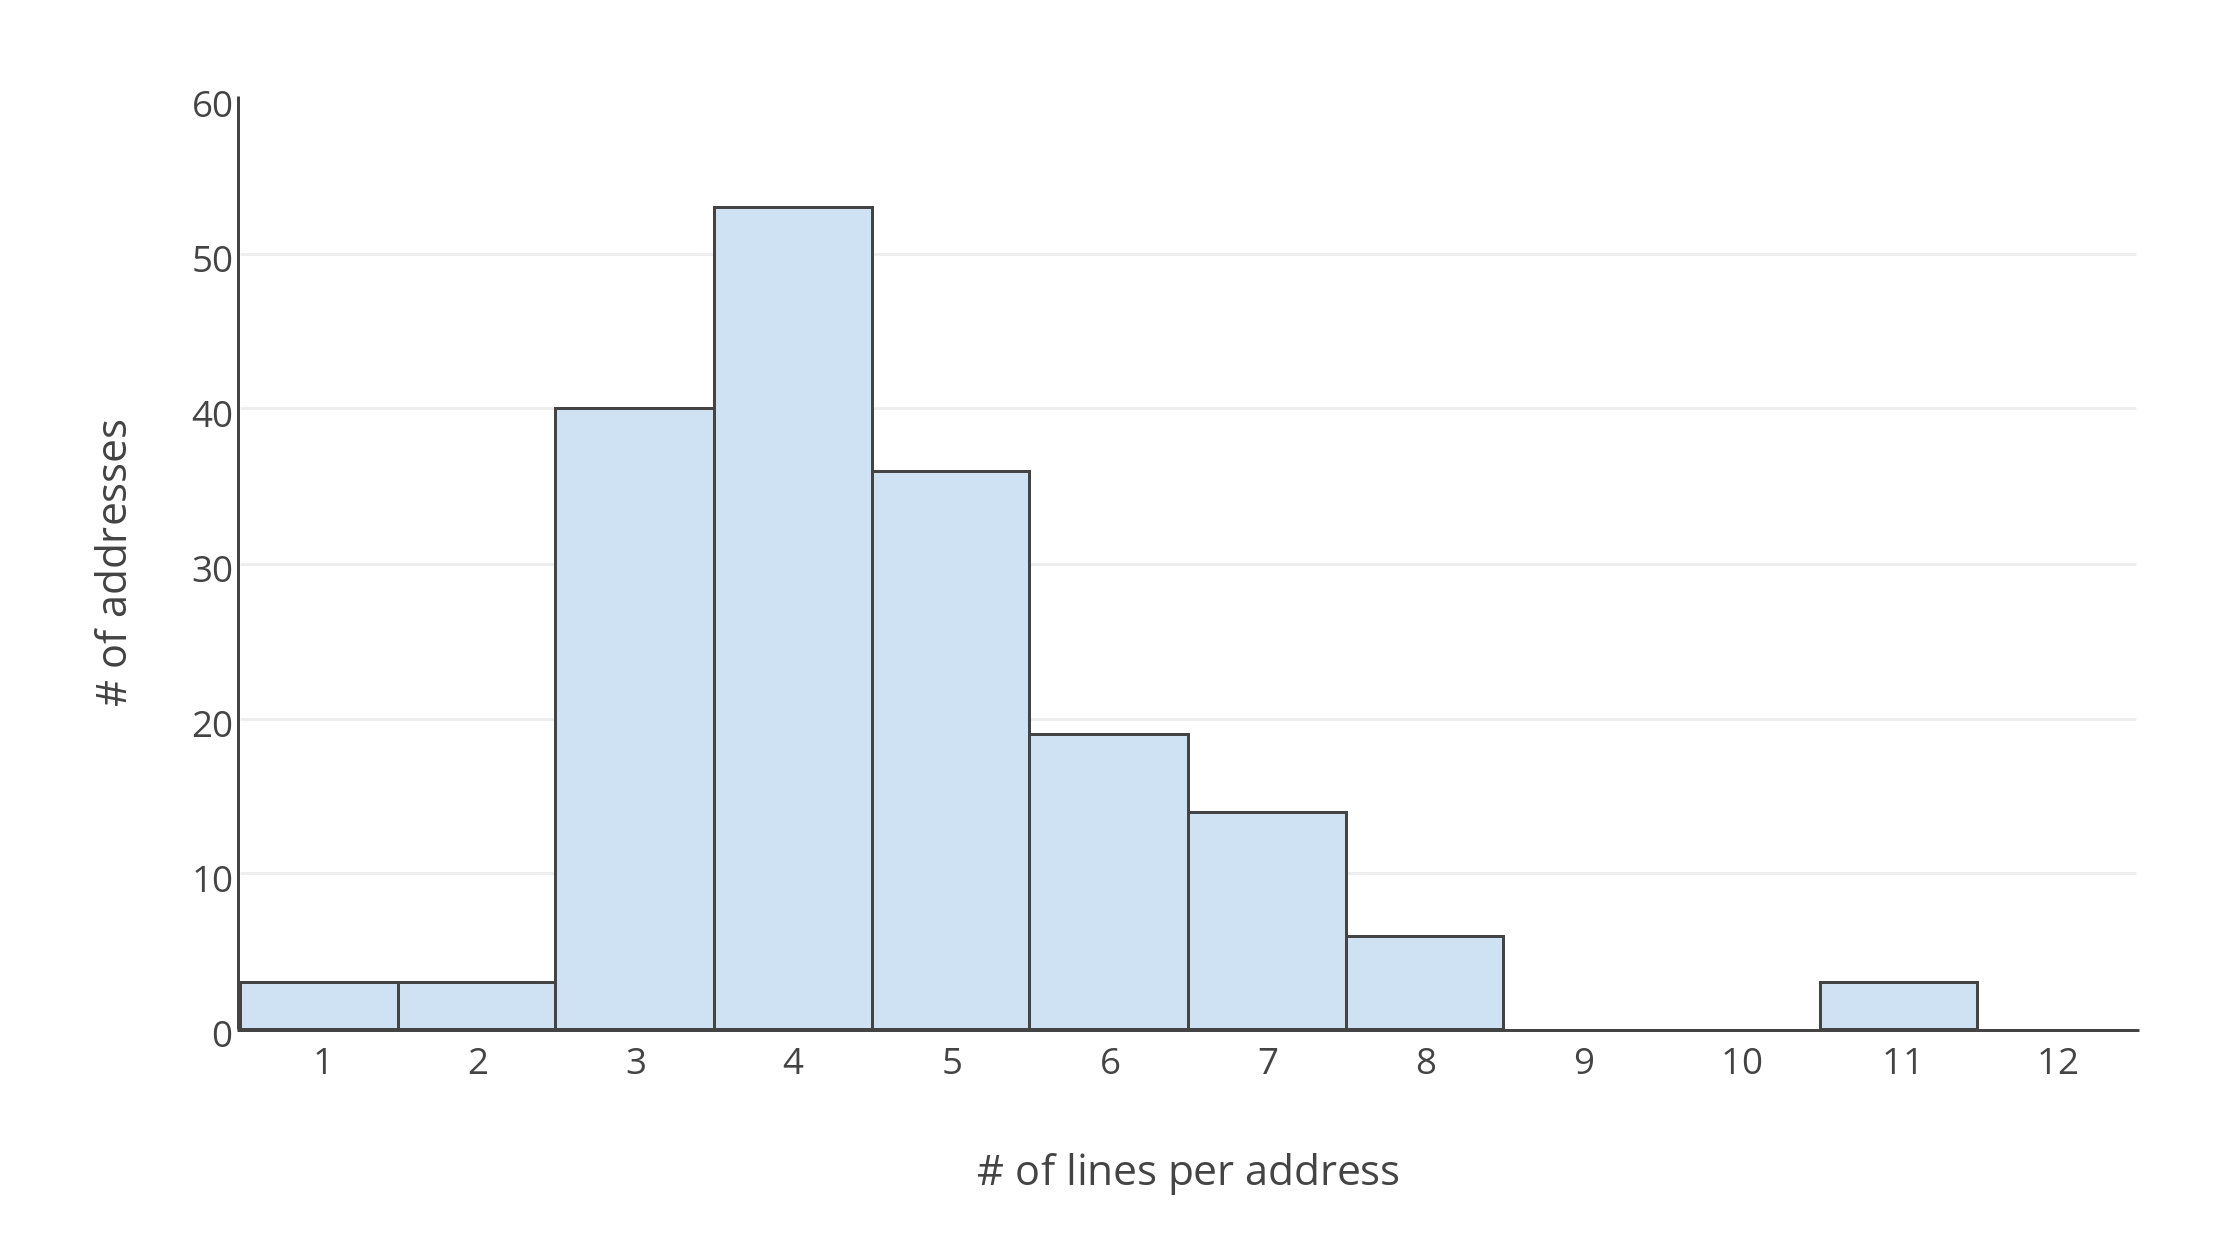
\includegraphics[width=0.8\textwidth]{../lib/images/address-lines-histogram}
	\caption{A histogram of the number of lines found in 178 addresses.\label{fig:addresslines}}
\end{center}
\end{figure}

\noindent Removing lines with 'department' or 'dept' was compared to an uninformed removal of the first line, and then the two approaches were combined (Figure \ref{fig:geoscatter}, points 2, 3 \& 4 respectively). Removing the first line gave the best compromise between a reduced hit rate but increased accuracy, so this approach was adopted in later approaches. Sending the last two lines of each address (Figure \ref{fig:geoscatter}, point 5) resulted in a low hit rate and low accuracy results, most likely due to the number of lines averaging around 4 (Figure \ref{fig:addresslines}), resulting in addresses that only specify the region and the country. It was surprising to see that the Places API would not geocode areas such as 'TN, USA', perhaps to focus on matching addresses as the primary use case of the service.\newline

\noindent After taking into account the data in Figure \ref{fig:geoscatter}, it could be seen that there would be a trade-off between hit rate and accuracy. For the three best-performing formats, 'no department', 'no first line' and 'second and third lines' (points 2, 3 \& 6, respectively), the distances were plotted to see the distribution of data (Figure \ref{fig:geoboxes}). With each formatting change from left to right, the dataset is expanded to include outliers of increasing frequency and inaccuracy. For example, the outlier 23 km away occurs in an address with the first line removed because the Places API returns the coordinates for an alternative campus. This type of inaccuracy, though sub-optimal, is permissible for this pilot version of the project. In contrast, an outlier 1336 km away occurs when only the second and third lines are used in one address; this kind of data is highly unrepresentative of the input data. These data informed the decision to format all addresses to exclude the first line and any email addresses.

\begin{figure}[!ht]
\begin{center}
	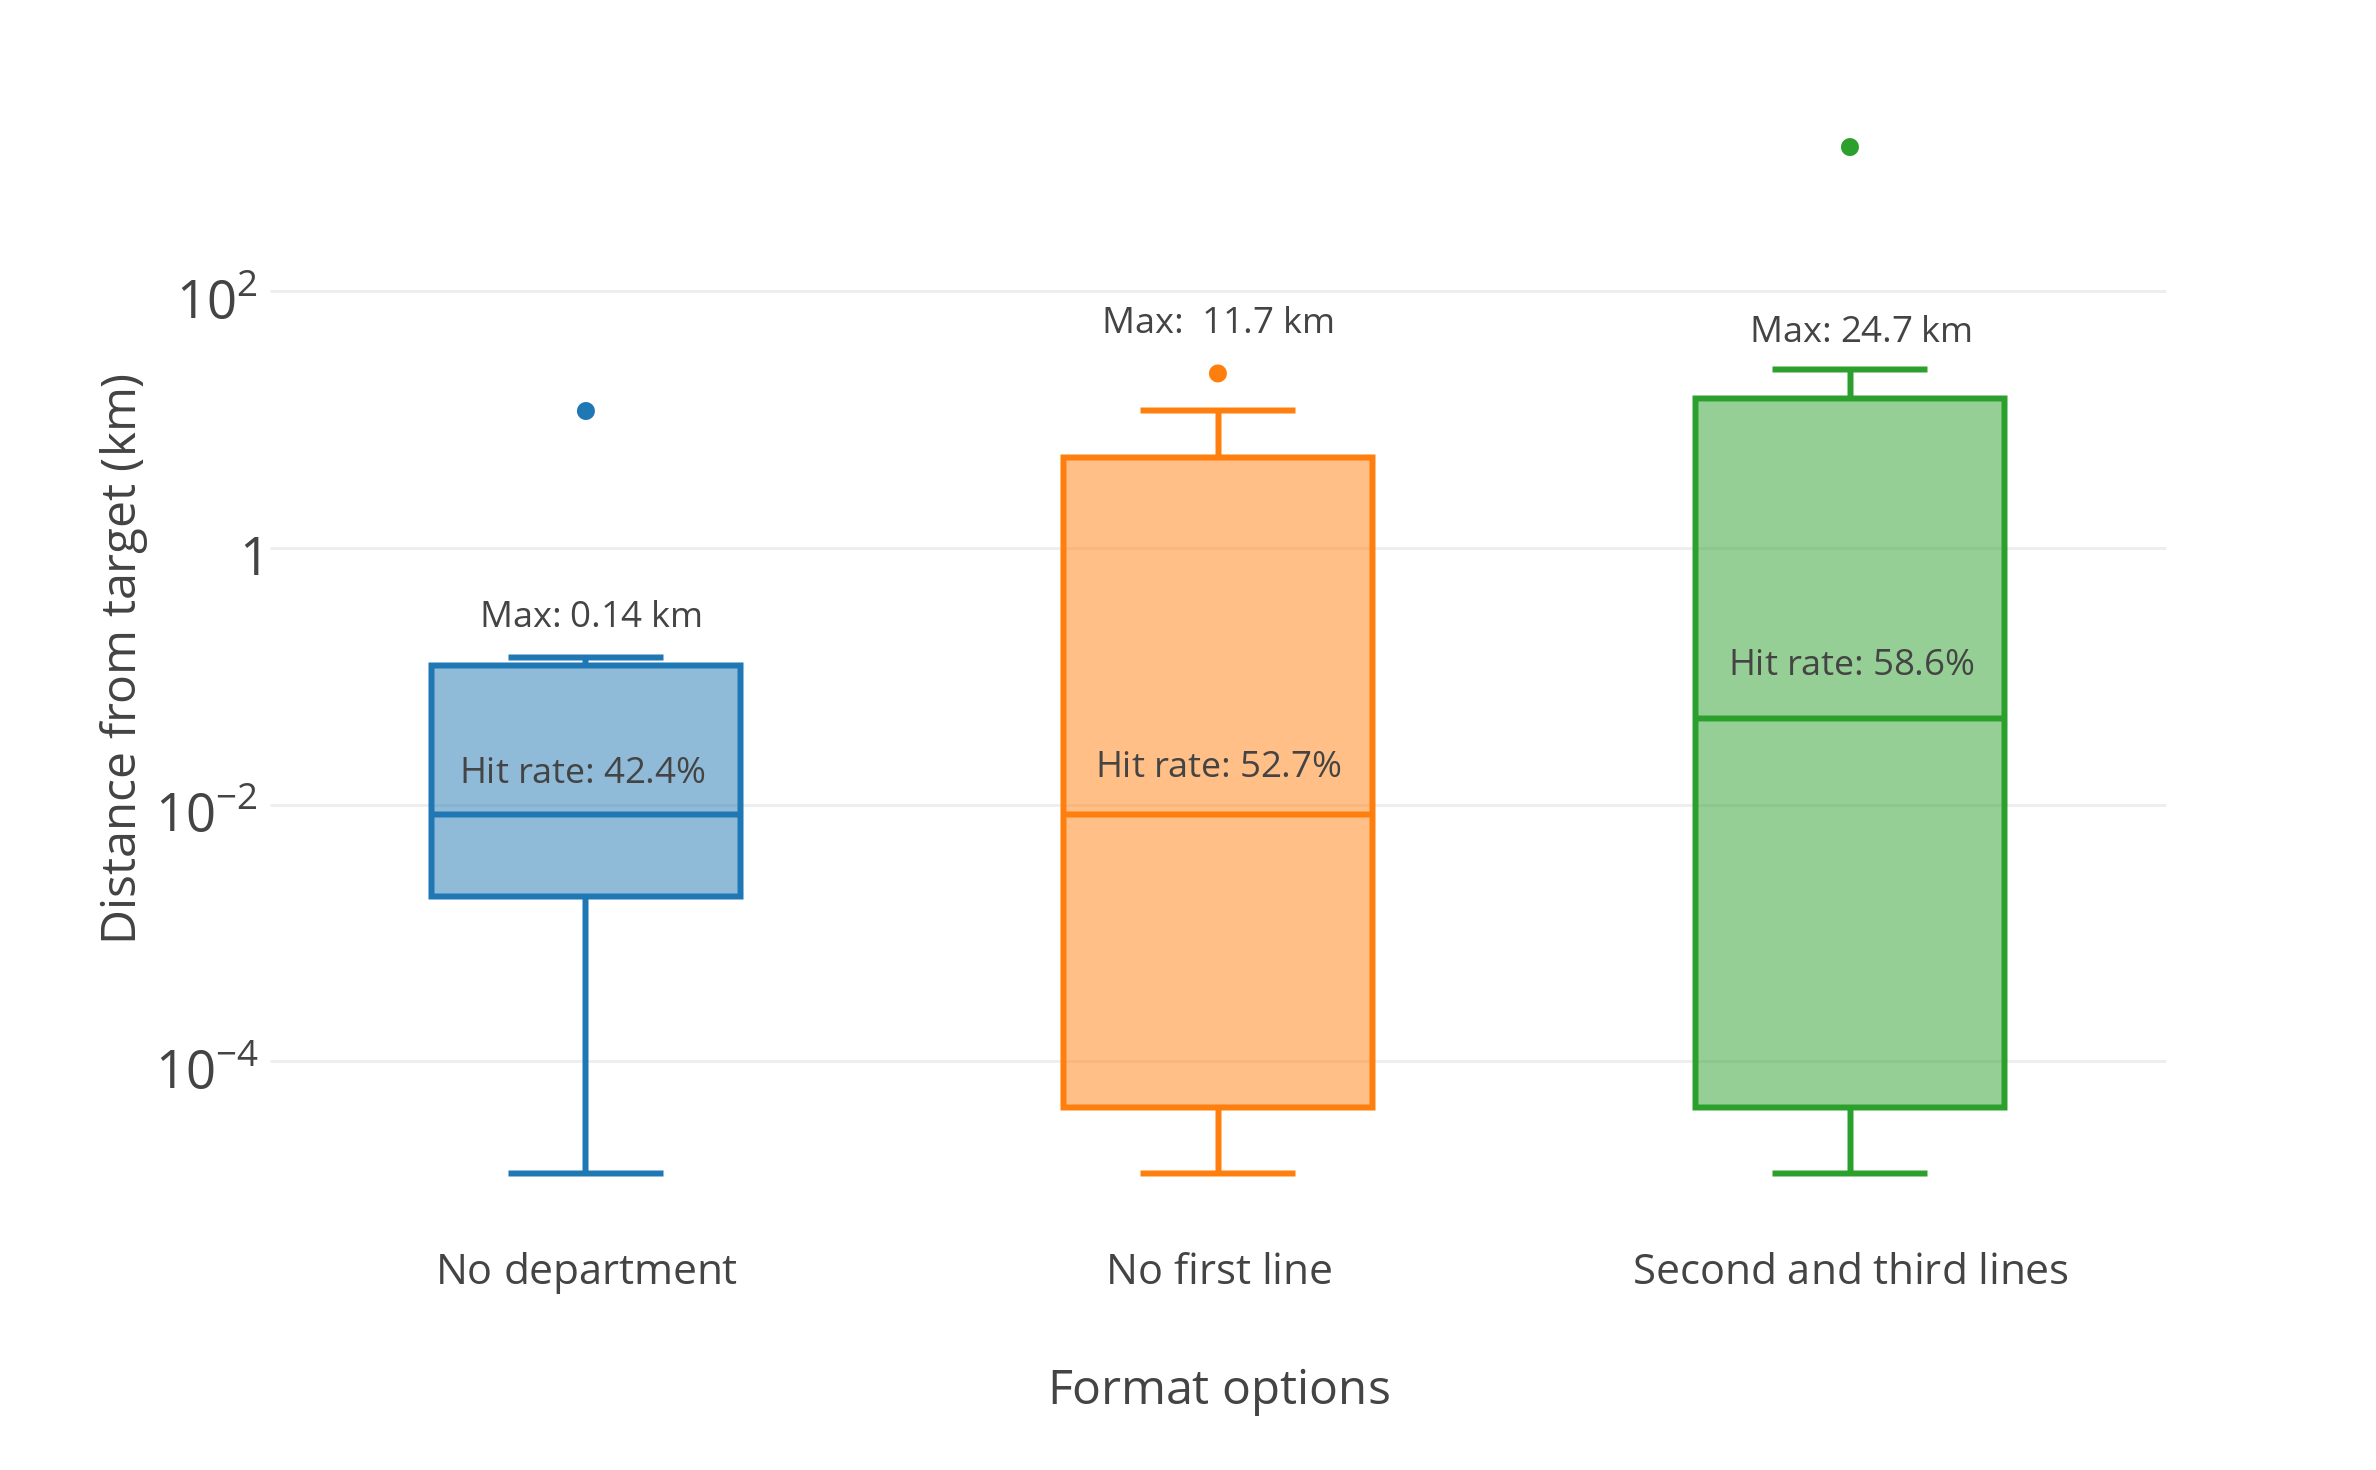
\includegraphics[width=0.8\textwidth]{../lib/images/distance-boxes}
	\caption{Box and Whisker diagrams for 3 formats with balanced hit rates and accuracies. Key values have been added to the diagram to allow clearer comparison, as the y-axis is log10 scale.\label{fig:geoboxes}}
\end{center}
\end{figure}

\subsection{Displaying data in the browser}
Explain more about what an SVG is.that can support the use of Scalable Vector Graphics (SVG) that are integral to this D3 application. Examples of this are as Mozilla Firefox 38+, Google Chrome 31+, or Internet Explorer 9+ (although manual scaling is required with the latter (CanIUse.com, \url{http://caniuse.com/#feat=svg})).

Research carried out in the planning stage of the project suggested that users are often looking for a paper they are already familiar with, and so another field is available for searching the author fields only. Increasing the specificity of this query with a simple interface allows the user to take full advantage of the additional functionality, whilst the search string is converted to an 'advanced' query server-side.

From here, a loading GIF is served to indicate to the user that the app is functional, and that results are incoming. this is important to improve the user's experience, and to prevent confusion at potentially long wait times.


\end{document}